\section{Data}

The advent of mobile sensing techniques makes it possible to develop urban geography from social media source. Complement the conventional census, social media brings the benefit of larger sampling frequency and higher disaggregate in terms of space and time, which reaches a wide range of individuals as well as collects the movement in human inactive time, such as the mid-night.

By Wechat, a widely used social media app we deployed the data collecting experiment in Shenzhen, one of the modernest metropolis in China. Figure~\ref{fig:app} shows the interfaces of the collecting app. Each individual hands in his or her personal characteristics from social, economic and deomgraphic aspects. For privacy issue, all detailed personal information are desensitized to categorical levels (Figure~\ref{fig:app}(b)). Also, individual is encouraged to upload trips (Figure~\ref{fig:app}(c)), including the information of start/end location and time, the traveling purpose and modes. A credit system is built up to retain the trip contribution of individuals and rewards those in the top contribution list (Figure~\ref{fig:app}(d)). 

\begin{figure}[htb!]
 \centering % avoid the use of \begin{center}...\end{center} and use \centering instead (more compact)
 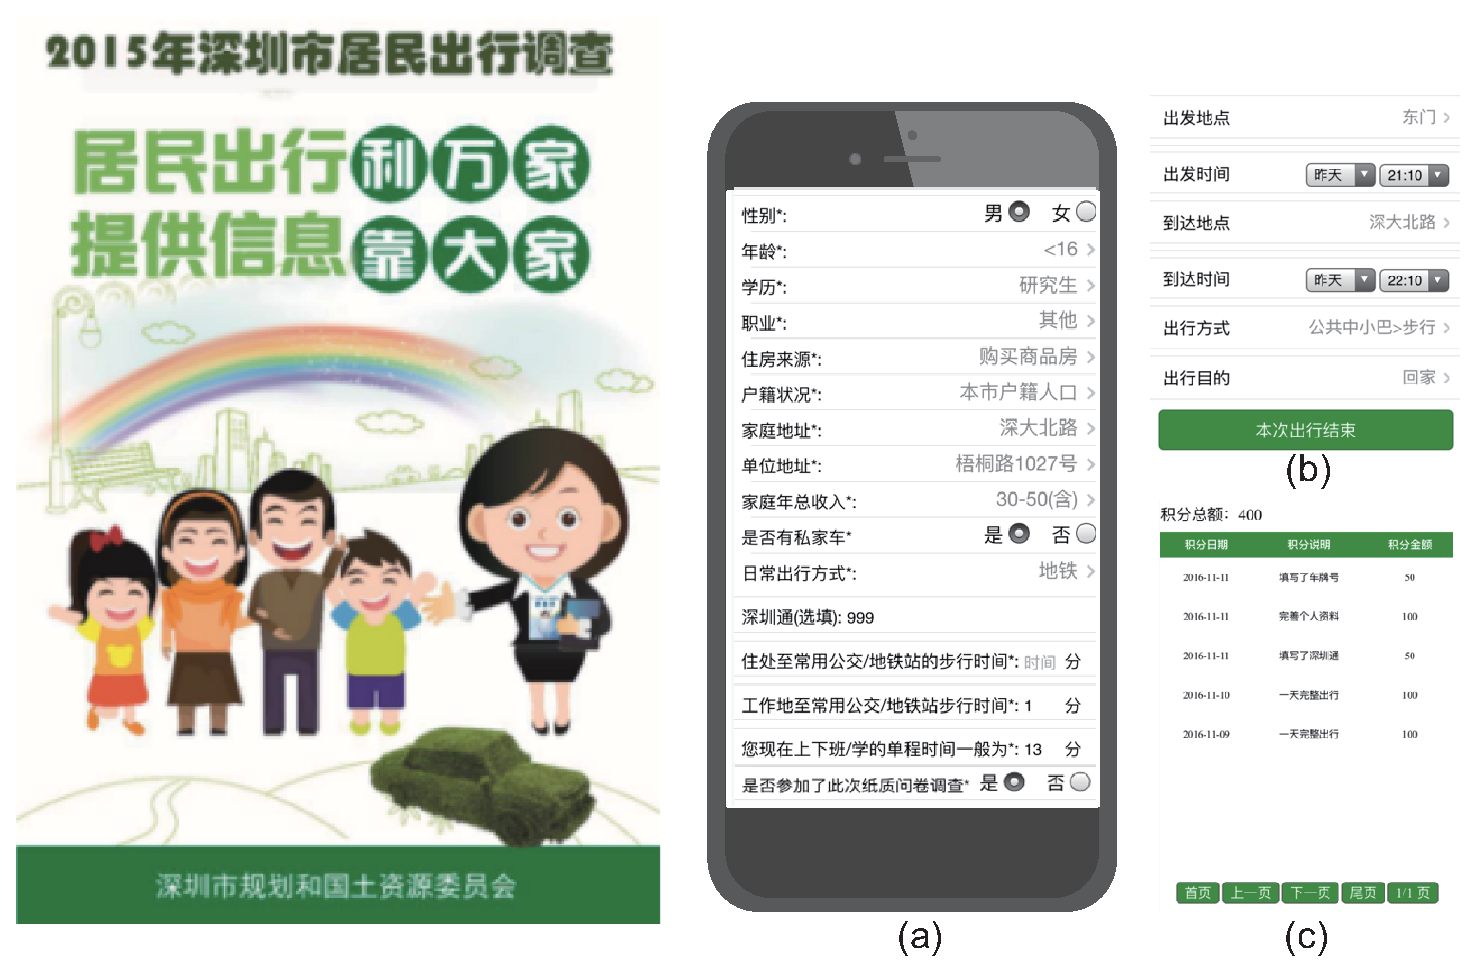
\includegraphics[width=\columnwidth]{pictures/survey_app}
 \caption{Collecting Interface: (a) welcome page; (b) personal characteristics collecting page; (c) trips collecting page; (d) credit system page}
 \label{fig:app}
\end{figure}


Over the releasing time period from June to October in 2015, 25481 individules were reached and XXX trips are collected, XX trips per individual. Figure~\ref{fig:data_over} lists the XX variables, falling into 8 domains. Those domains give a generalized depiction of the individual characteristics and serve as the ingredients for the analysis of urban dynamics over diverse people. 

Considering the caveat that self-selecting individuals are most unlikely to represent any clearly defined population~\cite{Longley2015}, a series of statistical analysis is performed to check whether it is rich enough to represent a wide range of human individuals in the city.


\begin{figure}[htb!]
 \centering % avoid the use of \begin{center}...\end{center} and use \centering instead (more compact)
 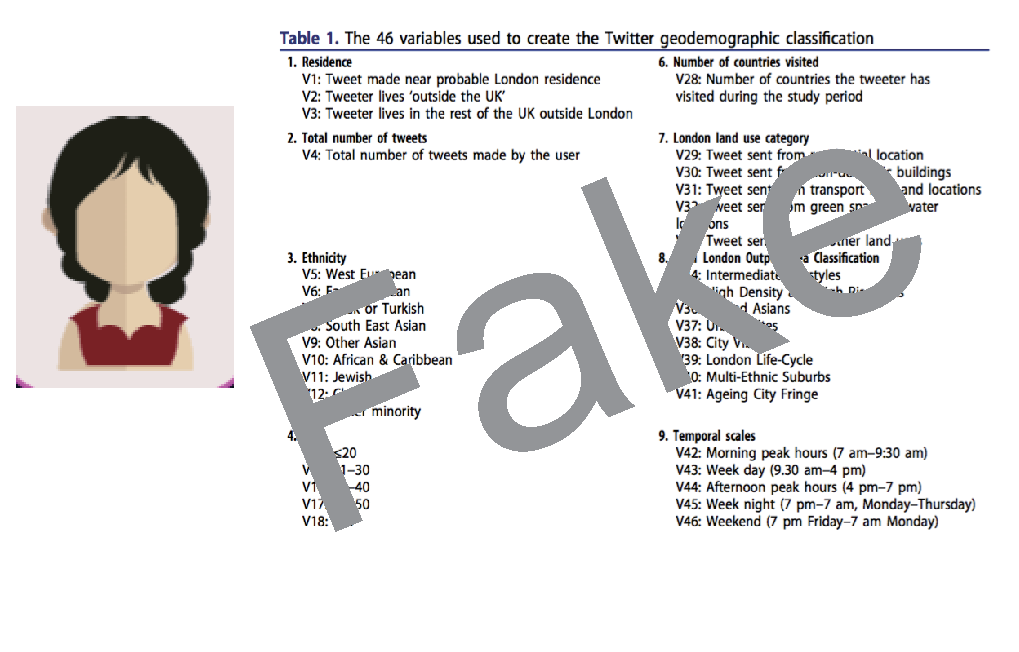
\includegraphics[width=\columnwidth]{pictures/data_over}
 \caption{Profile of Individual: XX variables falling into 8 domains enriches the analysis of urban dynamics}
 \label{fig:data_over}
\end{figure}

According to the 2015 Annual Census Statistics report~\footnote{http://www.sztj.gov.cn/xxgk/tjsj/pcgb/201606/t20160614\_3697000.htm}, people aging 15-64 occupy 83.23\% and the median age is 31.5. Shenzhen is majority of young people. 

\textit{Overview} Figure~\ref{fig:data_stat} shows samples covering almost all ages and age between 18 to 45. The 

\textit{Compared to Census} In the report (looking for some report), the penetration of mobile device is XXX, almost every XX people got a Mobile Phone in the urban. XX.  multiple social characteristics of a people is sampled, including income, education, etc. age and income distribution follows the social architecture. 


\begin{figure}[htb!]
 \centering % avoid the use of \begin{center}...\end{center} and use \centering instead (more compact)
 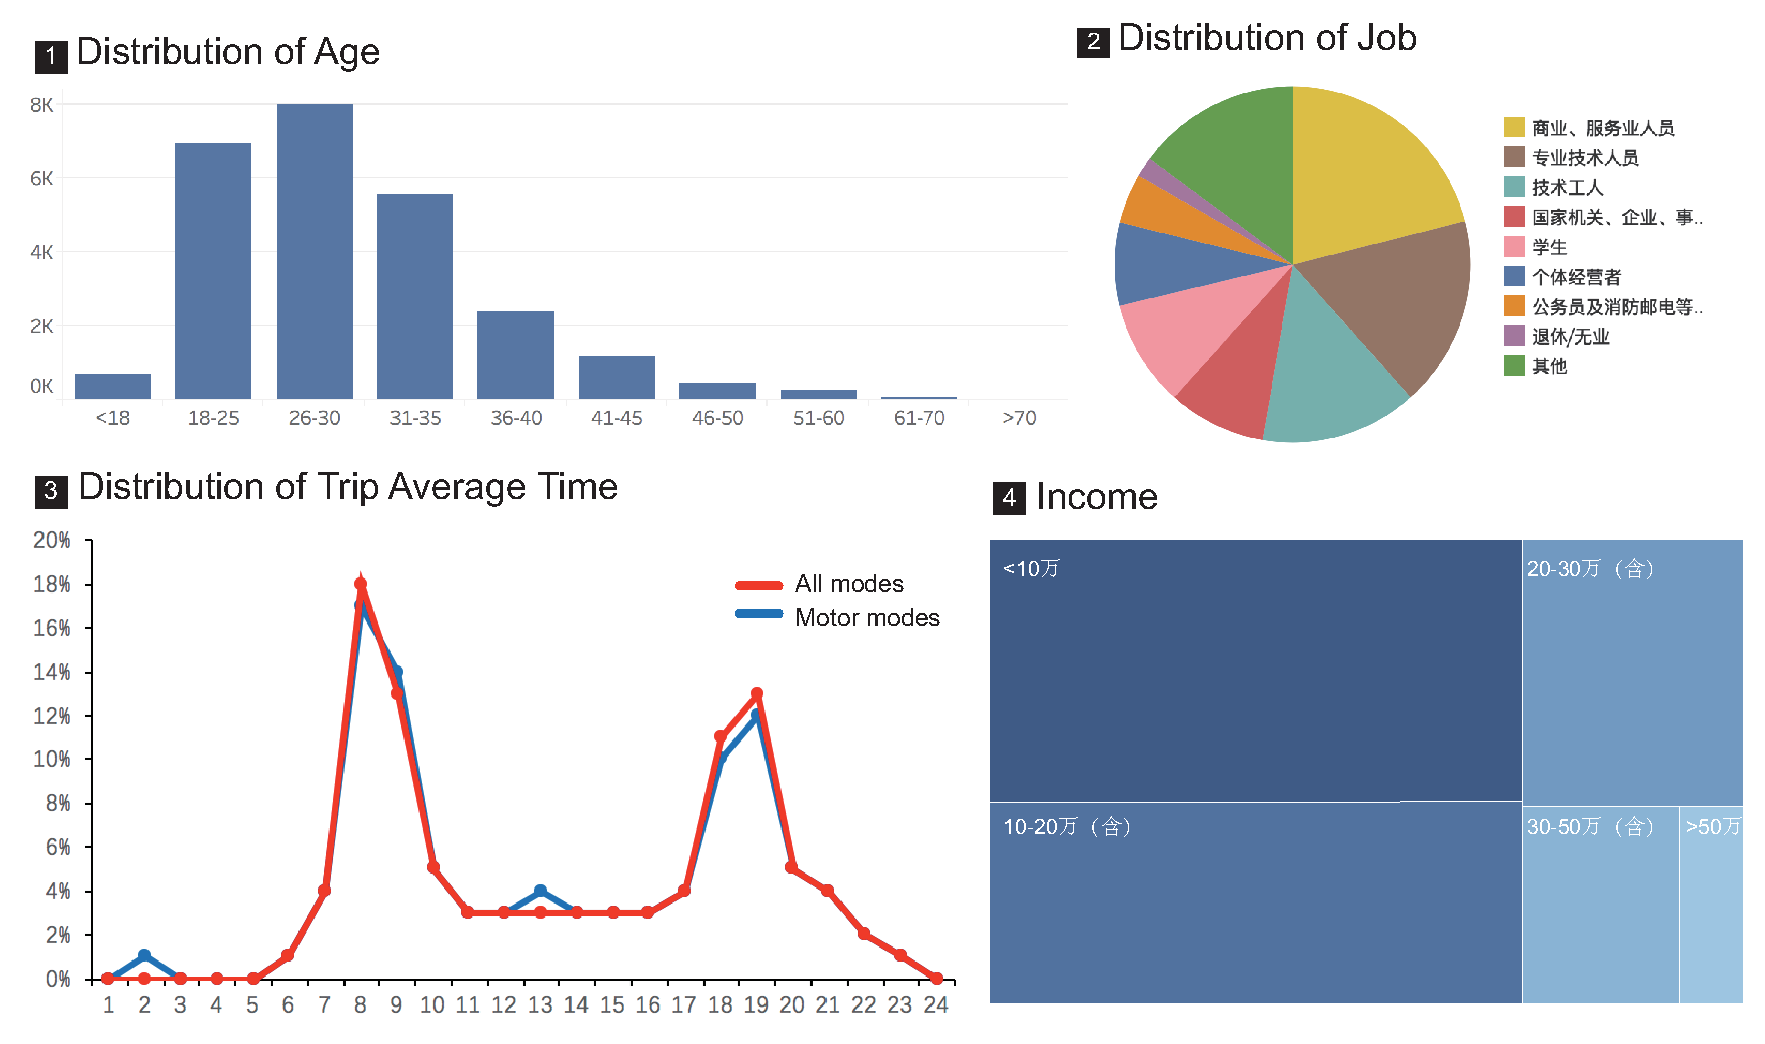
\includegraphics[width=\columnwidth]{pictures/data_detail}
 \caption{Statistical Overview of Social Characteristics}
 \label{fig:data_stat}
\end{figure}


